\documentclass[]{article}
\usepackage{lmodern}
\usepackage{graphicx}
\usepackage{adjustbox}
\usepackage{amssymb,amsmath}
\usepackage{ifxetex,ifluatex}
\usepackage{listings}
\usepackage[T1]{fontenc}
\usepackage[utf8]{inputenc}
\usepackage{microtype}
\usepackage[margin=1in]{geometry}
\usepackage{hyperref}
\usepackage{framed}
\usepackage{graphicx,grffile}
\usepackage{fancyvrb}
\usepackage{multirow}
\makeatletter
\def\maxwidth{\ifdim\Gin@nat@width>\linewidth\linewidth\else\Gin@nat@width\fi}
\def\maxheight{\ifdim\Gin@nat@height>\textheight\textheight\else\Gin@nat@height\fi}
\makeatother
% Scale images if necessary, so that they will not overflow the page
% margins by default, and it is still possible to overwrite the defaults
% using explicit options in \includegraphics[width, height, ...]{}
\setkeys{Gin}{width=\maxwidth,height=\maxheight,keepaspectratio}
\setlength{\parindent}{0pt}
\setlength{\parskip}{6pt plus 2pt minus 1pt}
\setlength{\emergencystretch}{3em}  % prevent overfull lines
\providecommand{\tightlist}{%
  \setlength{\itemsep}{0pt}\setlength{\parskip}{0pt}}

%%% Change title format to be more compact
\usepackage{titling}

% Create subtitle command for use in maketitle
\newcommand{\subtitle}[1]{
  \posttitle{
    \begin{center}\large#1\end{center}
    }
}

\setlength{\droptitle}{-2em}
  \title{MSAN 604 - Homework 2}
  \pretitle{\vspace{\droptitle}\centering\huge}
  \posttitle{\par}
  \author{Andre Guimaraes Duarte}
  \preauthor{\centering\large\emph}
  \postauthor{\par}
  \predate{\centering\large\emph}
  \postdate{\par}
  \date{November 17, 2016}
  
% Redefines (sub)paragraphs to behave more like section*s
\ifx\paragraph\undefined\else
\let\oldparagraph\paragraph
\renewcommand{\paragraph}[1]{\oldparagraph{#1}\mbox{}}
\fi
\ifx\subparagraph\undefined\else
\let\oldsubparagraph\subparagraph
\renewcommand{\subparagraph}[1]{\oldsubparagraph{#1}\mbox{}}
\fi

\usepackage{color}

%%%%%%%%%%%%%%%%%%%%%%%%%%%%%%%%%%%%%%%%%%%%%%%%%%%%%%%%%%%%%%%%%%%%%%%%%%%%%%%%%%%%%%%%%%%%%%%%%%%%%%%%%%%%%%%%%%%%%%%
\begin{document}
\null\hfill\begin{tabular}[t]{r@{}}
  \textbf{\LARGE Andre Guimaraes Duarte} \\
  \textbf{\Large 20406263}
\end{tabular}
%\maketitle

\begin{center}
\Huge
MSAN 604 - Homework 2

\Large
November 17, 2016

\normalsize
\end{center}

\section{Textbook Problems}
\paragraph{3.1}
Determine which of the following ARMA processes are causal and which of
them are invertible. (In each case $\{Z_t\}$ denotes white noise.)

a. $X_t + 0.2 X_{t-1} - 0.48 X_{t-2} = Z_t$

\color{blue}
We have 

$X_t + 0.2 X_{t-1} - 0.48 X_{t-2} = Z_t \Leftrightarrow \phi^2(B)X_t = Z_t$

with $\phi^2(z) = 1 + 0.2 z - 0.48 z^2$.

The roots of $\phi(z)$ are $z = \frac{-0.2 \pm \sqrt{(0.2)^2 + 4(0.48)^2}}{2(-0.48)} = \frac{0.2 \pm 1.4}{0.96}$. We get $z_1 = -1.25$ and $z_2 = 5/3$.

We have $|z_1| > 1$ and $|z_2| > 1$, so the process is \textbf{stationary}.

In addition, we have $\theta (z) = 1$. So the process is \textbf{invertible}.
\color{black}

b. $X_t + 1.9 X_{t-1} + 0.88 X_{t-2} = Z_t + 0.2 Z_{t-1} + 0.7 Z_{t-2}$

\color{blue}
We have

$X_t + 1.9 X_{t-1} + 0.88 X_{t-2} = Z_t + 0.2 Z_{t-1} + 0.7 Z_{t-2} \Leftrightarrow \phi^2(B)X_t = \theta^2(B)Z_t$

with $\phi^2(z) = 1 + 1.9 z + 0.88 z^2$ and $\theta^2(z) = 1 + 0.2 z + 0.7 z$.

The roots of $\phi^2(z)$ are $z = \frac{-1.9 \pm \sqrt{(1.9)^2 - 4(0.88)}}{2(0.88)} = \frac{-1.9 \pm \sqrt{0.09}}{1.76}$. We get $z_1 = -10/11$ and $z_2 = -5/4$.

We have $|z_1| < 1$, so the process is \textbf{not stationary}.

The roots of $\theta^2(z)$ are $z = \frac{-0.2 \pm \sqrt{(0.2)^2 - 4(0.7)}}{2(0.7)} = \frac{-0.2}{1.4} \pm i\frac{\sqrt{2.76}}{1.4}$.

We have $|z| = \sqrt{(0.2/1.4)^2 + (\sqrt{2.76}/1.4)^2} \simeq 1.2 > 1$. So the process is \textbf{invertible}.
\color{black}

c. $X_t + 0.6 X_{t-1} = Z_t + 1.2 Z_{t-1}$

\color{blue}
We have

$X_t + 0.6 X_{t-1} = Z_t + 1.2 Z_{t-1} \Leftrightarrow \phi(B)X_t = \theta(B)Z_t$

with $\phi(z) = 1 + 0.6 z$ and $\theta(z) = 1 + 1.2 z$.

The root of $\phi(z)$ is $z = \frac{-1}{0.6}$.

We have $|z| > 1$, so the process is \textbf{stationary}.

The root of $\theta(z)$ is $z = \frac{-1}{1.2}$.

We have $|z| < 1$, so the process is \textbf{not invertible}.
\color{black}

d. $X_t + 1.8 X_{t-1} + 0.81 X_{t-2} = Z_t$

\color{blue}
We have

$X_t + 1.8 X_{t-1} + 0.81 X_{t-2} = Z_t \Leftrightarrow \phi^2(B)X_t = Z_t$

with $\phi^2(z) = 1 + 1.8 z + 0.81 z^2$.

The root of $\phi^2(z)$ is $z = \frac{-1.8 \pm \sqrt{(1.8)^2 - 4(0.81)}}{2(0.81)} = \frac{-1.8 \pm \sqrt{3.24-3.24}}{1.62} = -10/9$.

We have $|z| > 1$, so the process is \textbf{causal}.

In addition, we have $\theta (z) = 1$. So the process is \textbf{invertible}.
\color{black}

e. $X_t + 1.6 X_{t-1} = Z_t - 0.4 Z_{t-1} + 0.04 Z_{t-2}$

\color{blue}
We have

$X_t + 1.6 X_{t-1} = Z_t - 0.4 Z_{t-1} + 0.04 Z_{t-2} \Leftrightarrow \phi(B)X_t = \theta^2(B)Z_t$

with $\phi(z) = 1 + 1.6 z$ and $\theta^2(z) = 1 - 0.4 z + 0.04 z^2$.

The root of $\phi(z)$ is $z = -1/1.6 < 1$, so the process is \textbf{not stationary}.

The root of $\theta(z)$ is $z = \frac{0.4 \pm \sqrt{(0.4)^2 - 4(0.04)}}{2(0.04)} = \frac{0.4 \pm \sqrt{0.16-0.16}}{0.08} = 5 > 1$. So the process is \textbf{invertible}.


\color{black}

\paragraph{1.10}
If $m_t = \sum^p_{k=0} c_k t^k,\ t = 0, \pm 1, \ldots$, show that $\nabla m_t$ is a polynomial of degree $p - 1$ in $t$ and hence that $\nabla^{p+1} m_t = 0$.

\color{blue}
We have $\nabla m_t = (1-B)m_t = m_t - m_{t-1} = \sum^p_{k=0} c_k t^k - \sum^p_{k=0} c_k (t-1)^k$.

It can easily be seen that the terms of order $p$ cancel each other out ($(c_p - c_p)t^p = 0$). 

In addition, the term of order $p-1$ is $p c_{p-1} \neq 0$. So the resulting polynomial is of degree $p-1$.

Therefore, every time the difference operator is applied to $m_t$, we get a polynomial of one less degree than $m_t$. As a result, we can have that $\nabla^{p} m_t$ is a polynomial of degree 0 (i.e. a constant). Therefore, we conclude that $\nabla^{p+1} m_t = 0$.

\color{black}

\paragraph{1.15}
Let $\{Y_t\}$ be a stationary process with mean zero and let $a$ and $b$ be constants.

a. If $X_t = a + bt + s_t + Y_t$, where $s_t$ is a seasonal component with period 12, show that $\nabla \nabla_{12} X_t = (1 - B)(1 - B^{12})X_t$ is stationary and express its autocovariance function in terms of that of $\{Y_t\}$.

\color{blue}
Let's call $W_t = \nabla \nabla_{12} X_t$.

We have

\begin{tabular}{ccl}
$W_t$ & = & $\nabla \nabla_{12} X_t$\\
      & = & $(1-B)(1-B^{12})X_t$\\
      & = & $(1-B)(X_t - X_{t-12})$\\
      & = & $X_t - X_{t-12} - X_{t-1} + X_{t-13}$\\
      & = & $a+bt+s_t+Y_t -a-b(t-12)-s_{t-12}-Y_{t-12} -a-b(t-1)-s_{t-1}-Y_{t-1} +a+b(t-13)+s_ {t-13}+Y_{t-13}$\\
      & = & $Y_t - Y_{t-1} - Y_{t-12} + Y_{t-13}$
\end{tabular}

So we have $\mu_W(t) = E[W_t] = E[Y_t - Y_{t-1} - Y_{t-12} + Y_{t-13}] = 0$ does not depend on $t$.

We also have

\begin{tabular}{ccl}
$\gamma_W(t, t+h)$ & = & $Cov(W_t, W_{t+h})$\\
& = & $Cov(Y_t - Y_{t-1} - Y_{t-12} + Y_{t-13}, Y_{t+h} - Y_{t+h-1} - Y_{t+h-12} + Y_{t+h-13})$\\
& = & $Cov(Y_t, Y_{t+h}) - Cov(Y_t, Y_{t+h-1}) - Cov(Y_t, Y_{t+h-12}) + Cov(Y_t, Y_{t+h-13})$\\
&  & - $Cov(Y_{t-1}, Y_{t+h}) + Cov(Y_{t-1}, Y_{t+h-1}) + Cov(Y_{t-1}, Y_{t+h-12}) - Cov(Y_{t-1}, Y_{t+h-13})$\\
& & - $Cov(Y_{t-12}, Y_{t+h}) + Cov(Y_{t-12}, Y_{t+h-1}) + Cov(Y_{t-12}, Y_{t+h-12}) - Cov(Y_{t-12}, Y_{t+h-13})$\\
& & + $Cov(Y_{t-13}, Y_{t+h}) - Cov(Y_{t-13}, Y_{t+h-1}) - Cov(Y_{t-13}, Y_{t+h-12}) + Cov(Y_{t-13}, Y_{t+h-13})$\\
& = & $\gamma_Y(h) - \gamma_Y(h-1) - \gamma_Y(h-12) + \gamma_Y(h-13)$\\
& & $- \gamma_Y(h+1) + \gamma_Y(h) + \gamma_Y(h-11) - \gamma_Y(h-12)$\\
& & $- \gamma_Y(h+12) + \gamma_Y(h+11) + \gamma_Y(h) - \gamma_Y(h-1)$\\
& & $+ \gamma_Y(h+13) - \gamma_Y(h+12) - \gamma_Y(h+1) + \gamma_Y(h)$\\
& = & $4\gamma_Y(h) -2\gamma_Y(h-1) -2\gamma_Y(h-12) +\gamma_Y(h-13)$\\
& & $-2\gamma_Y(h+1) +\gamma_Y(h-11) -2\gamma_Y(h+12) +\gamma_Y(h+11) +\gamma_Y(h+13)$
\end{tabular}

So we get that $\gamma_W(t, t+h)$ does not depend on $t$.

Therefore, we can conclude that the process $\{W_t\}$ is stationary.

\color{black}

b. If $X_t = (a + bt)s_t + Y_t$, where $s_t$ is a seasonal component with period 12, show that $\nabla^2_{12} X_t = (1 - B^{12})^2 X_t$ is stationary and express its autocovariance function in terms of that of $\{Y_t\}$.

\color{blue}
Let's call $Z_t = \nabla_{12}^2 X_t$.

We have

\begin{tabular}{ccl}
$Z_t$ & = & $\nabla_{12}^2 X_t$\\
      & = & $(1-B^{12})^2X_t$\\
      & = & $(1-B^{12})(1-B^{12})X_t$\\
      & = & $(1-B^{12})(X_t - X_{t-12})$\\
      & = & $X_t - X_{t-12} - X_{t-12} + X_{t-24}$\\
      & = & $X_t - 2X_{t-12} + X_{t-24}$\\
      & = & $(a+bt)s_t+Y_t -2((a+b(t-12))s_{t-12}+Y_{t-12}) +(a+b(t-24))s_{t-24} + Y_{t-24}$\\
      & = & $a(s_t-2s_{t-12}+s_{t-24}) + b(ts_t-2(t-12)s_{t-12}+(t-24)s_{t-24})+Y_t-2Y_{t-12}+Y_{t-24}$\\
      & = & $Y_t-2Y_{t-12}+Y_{t-24}$
\end{tabular}

So we have $\mu_Z(t) = E[Z_t] = E[Y_t-2Y_{t-12}+Y_{t-24}] = 0$ does not depend on $t$.

We also have

\begin{tabular}{ccl}
$\gamma_Z(t, t+h)$ & = & $Cov(Z_t, Z_{t+h})$\\
& = & $Cov(Y_t-2Y_{t-12}+Y_{t-24}, Y_{t+h}-2Y_{t+h-12}+Y_{t+h-24})$\\
& = & $Cov(Y_t, Y_{t+h}) -2Cov(Y_t, Y_{t+h-12}) +Cov(Y_t, Y_{t+h-24})$\\
&   & $-2Cov(Y_{t-12}, Y_{t+h}) +4Cov(Y_{t-12}, Y_{t+h-12}) -2Cov(Y_{t-12}, Y_{t+h-24})$\\
&   & $+ Cov(Y_{t-24}, Y_{t+h}) -2Cov(Y_{t-24}, Y_{t+h-12}) +Cov(Y_{t-24}, Y_{t+h-24})$\\
& = & $\gamma_Y(h) -2\gamma_Y(h-12) +\gamma_Y(h-24)$\\
&   & $-2\gamma_Y(h+12) +4\gamma_Y(h) -2\gamma_Y(h-12)$\\
&   & $+\gamma_Y(h+24) -2\gamma_Y(h+12) +\gamma_Y(h)$\\
& = & $6\gamma_Y(h) -4\gamma_Y(h-12) +\gamma_Y(h-24) -4\gamma_Y(h+12) +\gamma_Y(h+24)$
\end{tabular}

So we get that $\gamma_Z(t, t+h)$ does not depend on $t$.

Therefore, we can conclude that the process $\{Z_t\}$ is stationary.
\color{black}


\newpage
\section{Additional Problems}
\subsection{ARIMA fitting with the \texttt{LakeHuron} dataset.}
The \texttt{LakeHuron} dataset contains annual measurements of the level, in feet, of Lake Huron between 1875 and 1972.

(a) Take ordinary differences of the data until the resulting time series is suitably stationary, using the Augmented Dickey-Fuller Test to aid in your choice of d.

\color{blue}
We start by plotting the data and the ACF plot:

\begin{Verbatim}[frame=single]
# Plot original data
par(mfrow=c(2,1))
plot(LakeHuron)
acf(LakeHuron)
adf.test(LakeHuron)
\end{Verbatim}

\begin{figure}[!ht]
\centering
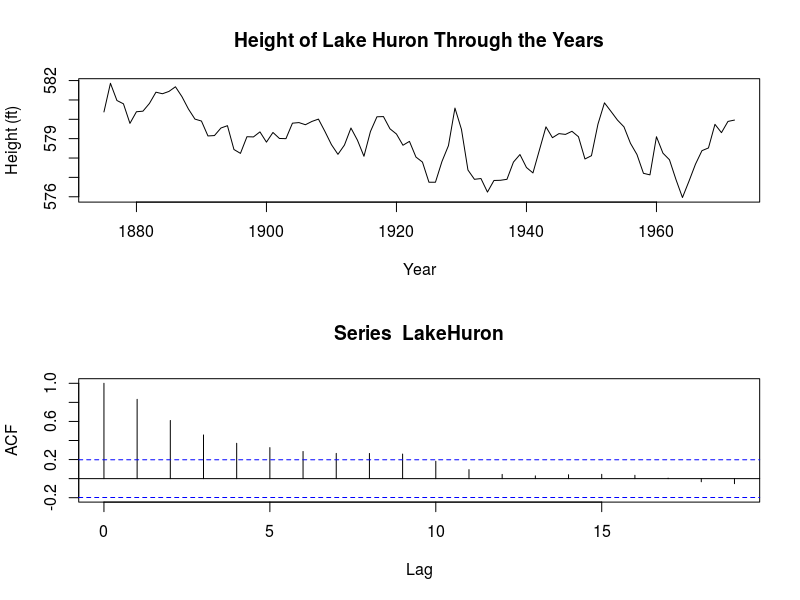
\includegraphics[width=.8\textwidth]{huronplot.png}
\caption{Plot of the data and ACF plot.}
\label{huronplot}
\end{figure}


We get the plots shown in Figure \ref{huronplot}, where we can see that the process is clearly not stationary. Indeed, the Augmented Dickey-Fuller test produces a p-value of 0.254. So we do not reject the null hypothesis that the time series is not stationary. Therefore, we try differencing once and look at the result:

\begin{Verbatim}[frame=single]
# Difference once
LakeHuron1 <- diff(LakeHuron)
plot(LakeHuron1)
acf(LakeHuron1)
adf.test(LakeHuron1)
\end{Verbatim}

\begin{figure}[!ht]
\centering
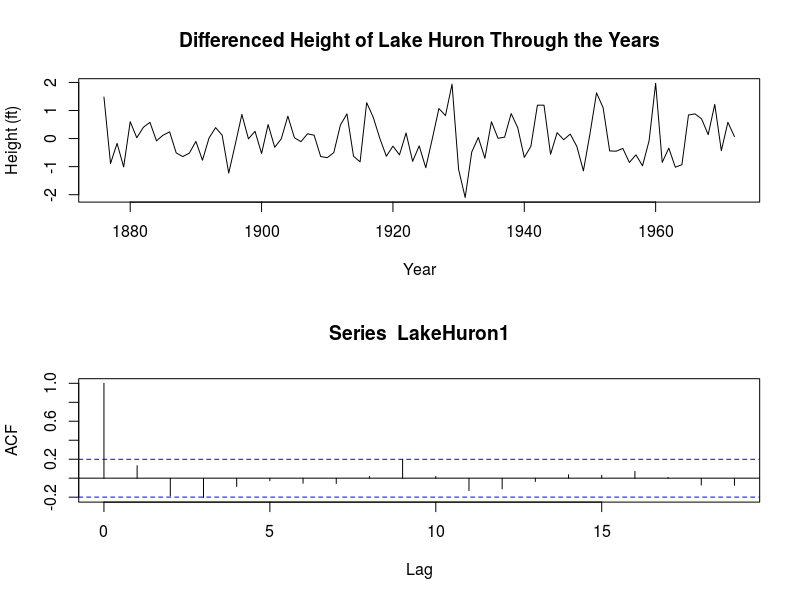
\includegraphics[width=.8\textwidth]{huron1plot.png}
\caption{Plot of the 1-differenced data and ACF plot.}
\label{huron1plot}
\end{figure}


We get the plots shown in Figure \ref{huron1plot}, where the process seems stationary. Indeed, the Augmented Dickey-Fuller test now produces a p-value $< 0.01$, so we reject the null hypothesis and conclude that the time series is stationary. We do not need to difference again. We conclude that $d=1$.

\color{black}

(b) Fit an $AR(1)$ model to the d-differenced \texttt{LakeHuron} data, using maximum likelihood estimation.

\color{blue}
We fit an AR(1) model to the 1-differenced data:

\begin{Verbatim}[frame=single]
m1 <- arima(LakeHuron1, order = c(1,0,0))
\end{Verbatim}

For this model, we get $\hat{\sigma}^2 = 0.5452$, log likelihood = -108.23, and aic = 222.45.
\color{black}

(c) Fit an $AR(2)$ model to the d-differenced \texttt{LakeHuron} data, using maximum likelihood estimation.

\color{blue}
We fit an AR(1) model to the 1-differenced data:

\begin{Verbatim}[frame=single]
m2 <- arima(LakeHuron1, order = c(1,0,0))
\end{Verbatim}

For this model, we get $\hat{\sigma}^2 = 0.5188$, log likelihood = -105.87, and aic = 219.74.
\color{black}

(d) Perform a likelihood ratio test comparing the $AR(1)$ and $AR(2)$ models and state
whether or not the null hypothesis is rejected.

\color{blue}
We perform a Likelihood Ratio Test to compare the two models. Here, the null model is \texttt{m1}, and the alternative model is \texttt{m2}:

\begin{Verbatim}[frame=single]
# Compare the two models using LRT
D <- -2*(m2$loglik - m1$loglik)
pval <- 1-pchisq(D,1)
print(c("Test Statistic:",round(D,4),"P-value:",round(pval,4)))
\end{Verbatim}

We get a p-value of 1, so we do not reject the null hypothesis that the two models fit equally well.
\color{black}

(e) Using your results from (d) and an assessment of $AIC$ and $\hat{sigma}^2$ for each model, state which model you deem to be “optimal” and briefly explain this choice.

\color{blue}
From the result in (d), we are inclined to choose the simpler model \texttt{m1}. By comparing $AIC$ and $\hat{sigma}^2$, we see that they are slightly higher for \texttt{m1}. However, the difference does not seem enough to warrant using the AR(2) model in this case.
\color{black}

(f) Using appropriate formal and informal residual diagnostics, investigate whether the “optimal” model you’ve chosen in (e) satisfies the following assumptions
\begin{itemize}
  \item Zero-Mean
  \item Homoscedasticity
  \item Zero-Correlation
  \item Normality
\end{itemize}

\color{blue}
We start by extracting the residuals from the model:

\begin{Verbatim}[frame=single]
# Residual diagnostics
e <- m1$residuals # residuals
r <- e/sqrt(m1$sigma2) # standardized residuals
\end{Verbatim}

Then, we plot the residuals against time. The horizontal line at 0 makes it easier to see whether the data seems to have zero-mean.
\begin{Verbatim}[frame=single]
# Plot residuals vs t
par(mfrow=c(2,1))
plot(e, main="Residuals vs t", ylab="")
abline(h=0, col="red")
plot(r, main="Standardized Residuals vs t", ylab="")
abline(h=0, col="red")

# test whether residuals have zero mean
t.test(e)
\end{Verbatim}

\begin{figure}[!ht]
\centering
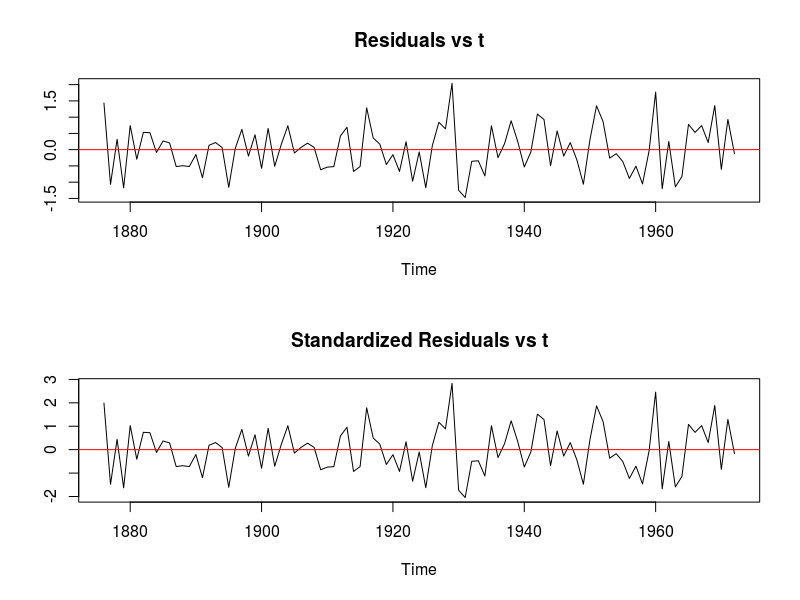
\includegraphics[width=.8\textwidth]{huronseq.png}
\caption{Sequential plot of residuals and standardized residuals.}
\label{huronseq}
\end{figure}

The plots in Figure \ref{huronseq} show that the process seems to have zero-mean. We can also say that it looks homoskedastic, and we can't discern any correlation nor outliers. The result from the t-test produces a p-value of 0.9765, so we do not reject the null hypothesis that the mean is zero.

In order to test Homoskedasticity, we split our data into four groups of similar length. Then we use Bartlett's and Levene's tests to check whether the variance in each group is statistically equal.
\begin{Verbatim}[frame=single]
# test for heteroscedasticity
par(mfrow=c(1,1))
plot(e, main="Residuals vs t", ylab="")
abline(v=c(1899,1923,1947), lwd=3, col="red")
group <- c(rep(1,24),rep(2,24),rep(3,24),rep(4,25))
levene.test(e,group) #Levene 
bartlett.test(e,group) #Bartlett 
\end{Verbatim}

\begin{figure}[!ht]
\centering
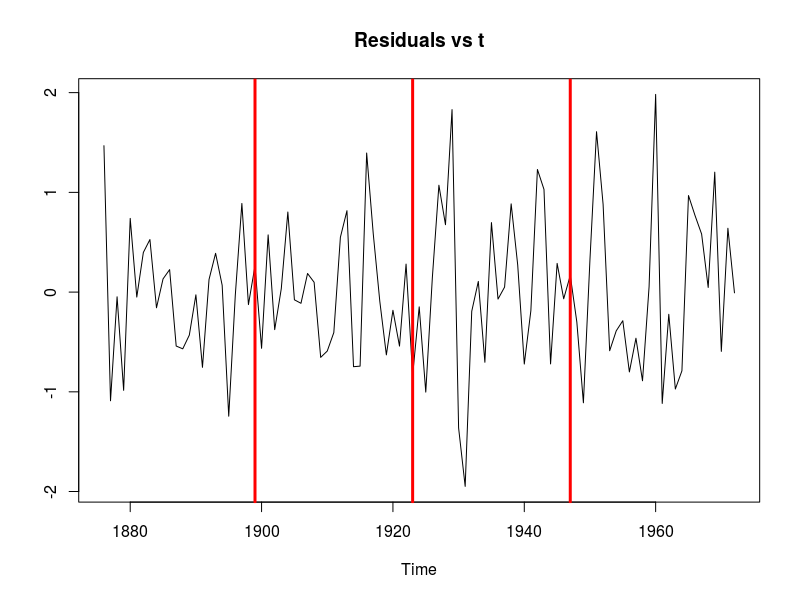
\includegraphics[width=.8\textwidth]{huronhomo.png}
\caption{Data splitting for homoskedasticity tests.}
\label{huronhomo}
\end{figure}

Bartlett's test produces a p-value of 0.2522, and Levene's test 0.1644. Therefore neither null hypothesis is rejected, and we conclude that the process is homoskedastic.

To formally check for uncorrelatedness, we use the Ljung-Box test:
\begin{Verbatim}[frame=single]
# test for uncorrelatedness / randomness
tsdiag(m1)
\end{Verbatim}

\begin{figure}[!ht]
\centering
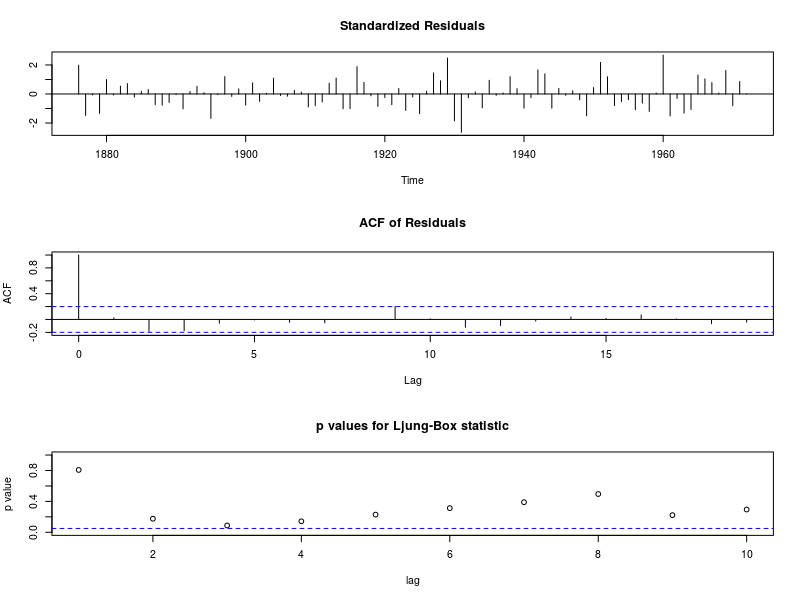
\includegraphics[width=.8\textwidth]{huronljung.png}
\caption{Plots for the Ljung-Box test.}
\label{huronljung}
\end{figure}

The plots in Figure \ref{huronljung} indicate that the data is random/uncorrelated.

Finally, we need to verify if the residuals are normally distributed, since we used Maximum Likely Estimators:
\begin{Verbatim}[frame=single]
# test for normality
par(mfrow=c(1,1))
qqnorm(e, main="QQ-plot of Residuals")
qqline(e, col = "red")
shapiro.test(e) #SW test
\end{Verbatim}

\begin{figure}[!ht]
\centering
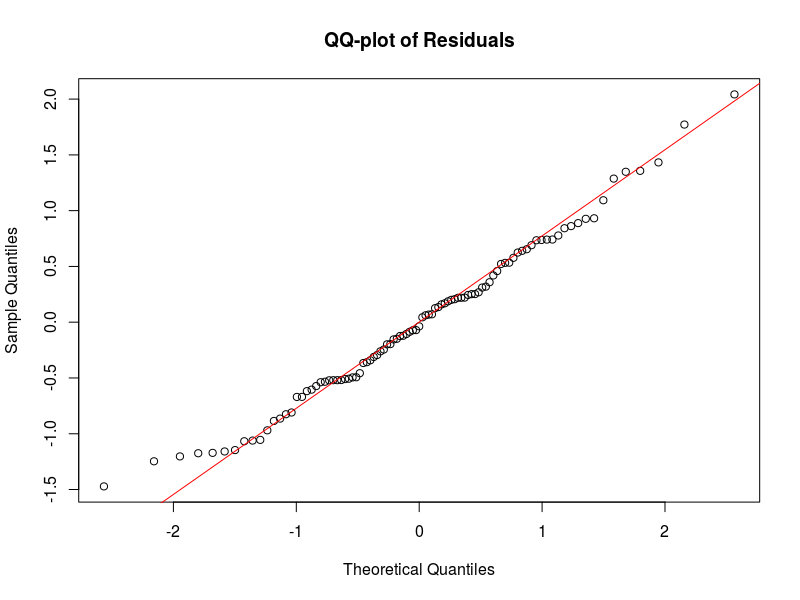
\includegraphics[width=.8\textwidth]{huronqq.png}
\caption{QQ-plot of the residuals.}
\label{huronqq}
\end{figure}

The QQ-plot in Figure \ref{huronqq} seems OK, and Shapiro-Wilk's test produces a p-value of 0.5982, so we do not reject the null hypothesis that the residuals are normally distributed.

All the residual diagnostics satisfy the assumptions, so we can accept the AR(1) model to model this process.
\color{black}

\newpage
\subsection{SARIMA fitting with the \texttt{beers.csv} dataset.}
The \texttt{beers.csv} dataset contains information on monthly Australian beer production,
in millions of litres, from January 1956 to August 1995.

(a) Using techniques discussed in class, fit (using maximum likelihood estimation) an “optimal” $SARIMA(p,d,q) \times (P,D,Q)$ model to the \texttt{beers.csv} time series, and justify your choice of $p, d, q, P, D, Q$ and $s$.

\color{blue}
We start by importing the data:
\begin{Verbatim}[frame=single]
# Load data
beer <- read.csv("beer.csv", header=T)
beer <- ts(beer, start = 1956, end = 1995, frequency = 12)
\end{Verbatim}
The term \texttt{frequency=12} is used to indicate that the data is separated by months.

Then, we can plot the process, as well as the ACF plot to determine stationarity and seasonality:
\begin{Verbatim}[frame=single]
# Plot the data
par(mfrow=c(2,1))
plot(beer)
acf(beer, lag.max = 144)
adf.test(beer)
\end{Verbatim}

\begin{figure}[!ht]
\centering
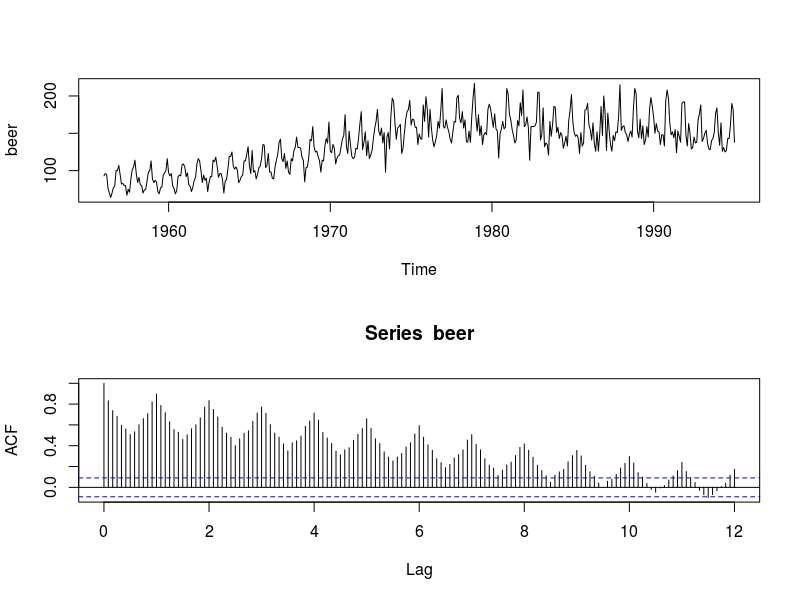
\includegraphics[width=.8\textwidth]{beer.png}
\caption{Plot of beer data set and ACF plot.}
\label{beer}
\end{figure}

The resulting plots shown in Figure \ref{beer} show that the time series is not stationary. However, the Augmented Dickey-Fuller test produces a significant p-value, which would suggest that we reject the null hypothesis that the process is not stationary.


Now, we difference again in order to remove the seasonality pattern.
\begin{Verbatim}[frame=single]
# Difference for seasonality (period=12)
beer1.12 <- diff(beer1, lag = 12)
plot(beer1.12)
acf(beer1.12, lag.max = 144)
\end{Verbatim}



\begin{Verbatim}[frame=single]

\end{Verbatim}


\color{black}

(b) Using appropriate formal and informal residual diagnostics, investigate whether the “optimal” model you’ve found in (a) satisfies the following assumptions
“optimal” model you’ve chosen in (e) satisfies the following assumptions
\begin{itemize}
  \item Zero-Mean
  \item Homoscedasticity
  \item Zero-Correlation
  \item Normality
\end{itemize}

\color{blue}

\color{black}

\end{document}
